\documentclass[10pt,a4paper]{article}

\usepackage[utf8]{inputenc}
\usepackage{microtype}
\usepackage[a4paper,margin=19mm,headheight=14pt]{geometry}
\usepackage{graphicx}
\usepackage{booktabs}
\usepackage{tabularx}
\usepackage{array}
\usepackage{multirow}
\usepackage{amsmath,amssymb}
\usepackage{enumitem}
\usepackage{caption}
\usepackage{subcaption}
\usepackage{float}
\usepackage{pdflscape}
\usepackage{fancyhdr}
\usepackage{titlesec}
\usepackage[hidelinks]{hyperref}
\usepackage{xurl}

\hypersetup{
  pdftitle={Adaptive Network Intrusion Detection and Pre-Milestone Early Warning: Phase 3},
  pdfauthor={Ibrahim Hussain},
  pdfsubject={Implementation and experimental evaluation},
  pdfkeywords={network intrusion detection, early warning, Zeek, temporal analysis, reproducibility}
}

\graphicspath{{figures/zeek/}}
\setlength{\parindent}{0pt}
\setlength{\parskip}{4pt}
\setlist[itemize]{leftmargin=*,nosep}
\setlist[enumerate]{leftmargin=*,itemsep=2pt,topsep=2pt}
\renewcommand{\arraystretch}{1.12}
\captionsetup{font=small,labelfont=bf}
\titleformat{\section}{\large\bfseries}{\thesection}{0.55em}{}
\titleformat{\subsection}{\normalsize\bfseries}{\thesubsection}{0.55em}{}

% \pagestyle{fancy}
% \fancyhf{}
% \lhead{Adaptive Network Intrusion Detection}
% \rhead{Phase 3 Implementation and Evaluation}
% \cfoot{\thepage}

\newcommand{\runone}{\texttt{cpu\_v3\_main\_v2\_20261115T164430Z}}
\newcommand{\runtwo}{\texttt{cpu\_v3\_main\_v2\_seed2\_20261115T165949Z}}
\newcommand{\sensorvalidated}{\texttt{SENSOR\_VALIDATED}}
\newcommand{\metric}[1]{\ensuremath{\mathbf{#1}}}

\begin{document}
\hypersetup{pageanchor=false}

{\centering \LARGE \bfseries Adaptive Network Intrusion Detection and Early Warning through Game-Theoretic Scenario Generation and Temporal
Network Analysis\par}
\vspace{5mm}
{\centering \large Ibrahim Hussain, Sameer Khan\par}
{\centering \large 23I-2626 , 23I-2517\par}
{\centering \large DS-A , DS-C\par}
{\centering \large Computer Networks\par}
\vspace{10mm}
% \vfill
\hypersetup{pageanchor=true}
\pagenumbering{arabic}

\begin{abstract}
This report presents a complete implementation and experimental evaluation of an adaptive network-intrusion-detection methodology in an isolated two-segment Docker laboratory. A controller generated bounded, harmless HTTP behaviours under fixed, uniform-random, and strategic EXP3-style scenario-selection policies. Ground-truth onset, escalation, and milestone times were recorded independently of the detectors. Traffic was observed through a restricted packet-capture sidecar, validated through a seven-check fail-closed gate, and converted to Zeek connection records. Whole episodes were split before causal window construction to prevent leakage. A transparent rate rule, Isolation Forest, Random Forest, and compact GRU were compared on one frozen test set containing both seen and held-out behaviour families. The strongest balanced result in the primary seed was obtained by the random-policy GRU: episode F1 $=0.889$, PR-AUC $=0.965$, strict early-warning coverage $=0.833$, and false-positive episode rate $=0.042$. The strategic-policy GRU was consistently the most conservative across two seeds, whereas policy coverage rankings varied between seeds. The study therefore establishes a reproducible collection, validation, and pre-milestone warning pipeline, while supporting a trade-off conclusion rather than an unsupported claim of a universally superior policy.
\end{abstract}

\textbf{Keywords:} network intrusion detection; early warning; temporal analysis; scenario selection; Zeek; reproducibility

\section{Research Objective and Contributions}

The objective was to implement and evaluate a network-centred methodology that measures both detection and warning before a declared later milestone. The central research question was:

\begin{quote}
Under a matched collection budget and a common frozen test set, does a bounded strategic scenario selector produce a detector that warns earlier, or with fewer false alarms, than fixed or uniform-random selection?
\end{quote}

The implementation contributes: (i) a contained cyber-range with independent controller ground truth; (ii) packet-level observation validated by strict Zeek processing; (iii) episode-level, leakage-safe preprocessing; (iv) matched baseline and temporal-model comparisons; (v) held-out-family evaluation; (vi) ablations of policy, temporal features, warning persistence, observation source, and scenario novelty; and (vii) an independent second-seed replication. The work intentionally makes no claim of real-malware, zero-day, graph-neural-network, future-stage-prediction, or production deployment performance.

\section{Implementation}

\subsection{Laboratory, containment, and data flow}

The laboratory comprised a scenario controller, client processes, a gateway, and two HTTP services joined by two Docker networks marked \texttt{internal=true}. Services dropped all Linux capabilities, enabled \texttt{no-new-privileges}, and used read-only root filesystems. The capture sidecar added only \texttt{NET\_RAW}, joined the gateway network namespace, and never used host networking or privileged mode. Requests were bounded to harmless HTTP messages of limited size; no public target, or autonomous propagation was used.

\begin{figure}[H]
\centering
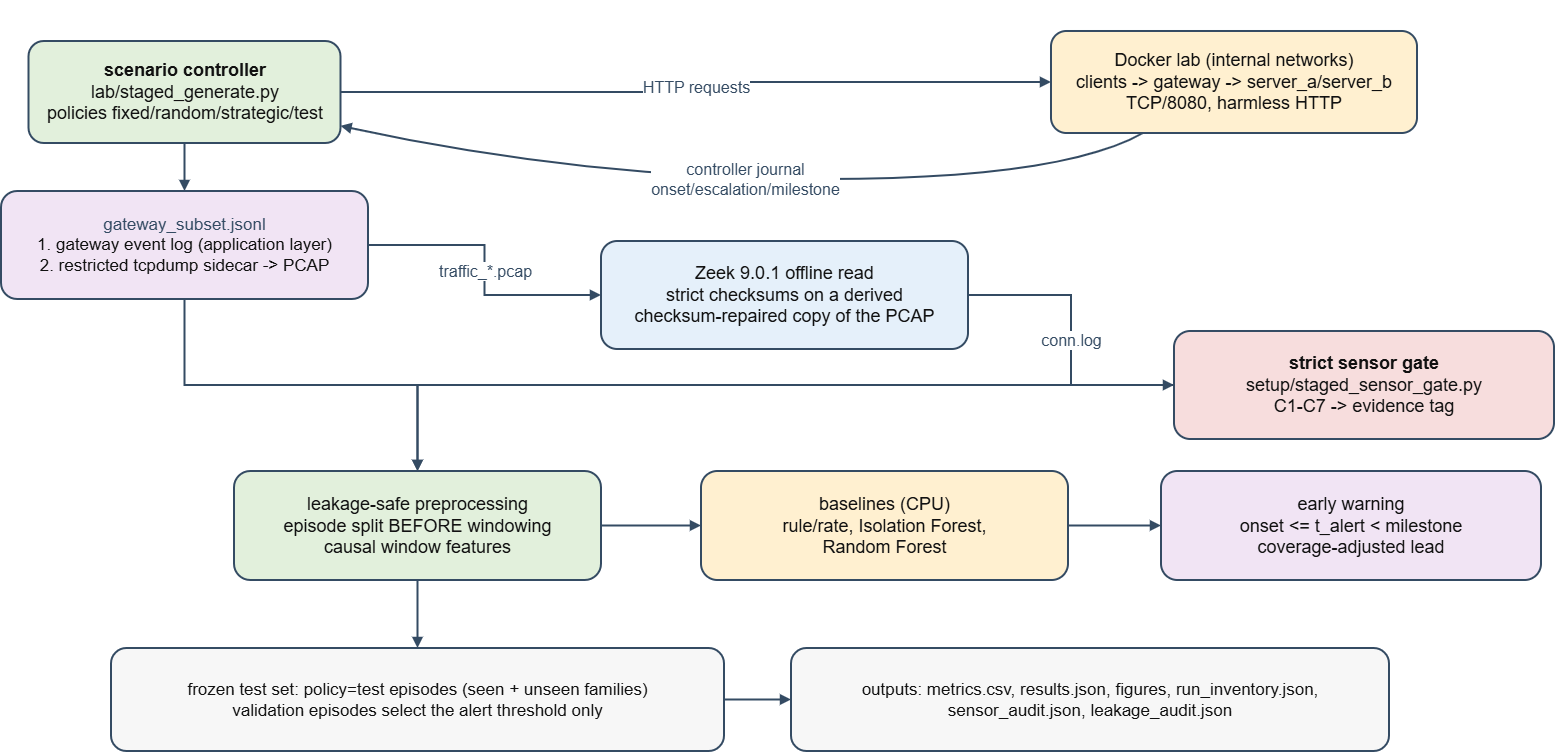
\includegraphics[width=\textwidth]{fig07_architecture.png}
\caption{Implemented architecture and evidence flow. The controller journal supplies ground truth; application and network sensors remain separate.}
\label{fig:architecture}
\end{figure}

The controller implemented four incident families and four benign variants. Development incident families were \texttt{rapid\_repeat}, \texttt{destination\_shift}, and \texttt{jittered\_burst}; \texttt{slow\_ramp} was held out from fitting and threshold selection. The four benign variants included a deliberately difficult \texttt{maintenance\_burst}. Fixed, uniform-random, and bounded strategic policies received equal collection budgets. The strategic selector used an EXP3-style update with a controller-derived heuristic reward; it was not detector feedback or a Nash-equilibrium method.

\subsection{Independent ground truth and warning semantics}

For each incident episode, the controller recorded onset (request 5), escalation (request 12), and milestone (request 19) before model execution, and enforced
\[
t_{\mathrm{start}} < t_{\mathrm{onset}} < t_{\mathrm{escalation}} < t_{\mathrm{milestone}} < t_{\mathrm{end}}.
\]
A warning was valid only when
\[
t_{\mathrm{onset}} \leq t_{\mathrm{alert}} < t_{\mathrm{milestone}},
\qquad
L_e=t_{\mathrm{milestone}}-t_{\mathrm{alert}}.
\]
Pre-onset alerts were not credited as warning, post-milestone alerts were late detections, and unwarned incidents received zero lead time in the coverage-adjusted mean. In addition to ordinary pre-milestone coverage, the evaluation reported \emph{strict first-alert coverage}: the first alert of any kind had to occur after onset and before the milestone. This prevents persistent pre-onset alarms from being misrepresented as early warning.

\section{Dataset Integrity and Experimental Protocol}

\subsection{Dataset and strict sensor validation}

The primary collection contained 192 episodes (96 benign and 96 incident), 3,840 gateway events, 107,628 packet records in a 13.4 MB PCAP, and 7,688 Zeek TCP connections. There were 20 requests per episode and two observed TCP connections per HTTP request (client--gateway and gateway--service). Causal window construction produced 6,336 windows: 3,168 training, 1,584 validation, and 1,584 test windows.

\begin{table}[H]
\centering
\caption{Fail-closed packet and sensor validation for the primary run.}
\small
\begin{tabularx}{\textwidth}{@{}p{9mm}Xr@{}}
\toprule
Check & Requirement & Result \\
\midrule
C1 & Completion marker, journal, gateway events, and at least one PCAP exist & Pass \\
C2 & PCAP is complete and parseable; packet count is plausible & Pass: 107,628 \\
C3 & Strict Zeek exits successfully and emits connection records & Pass: 7,688 \\
C4 & Expected TCP/8080 service traffic is present & Pass: 7,688/7,688 \\
C5 & Eligible flows have bidirectional byte visibility & Pass: 100\% \\
C6 & Zeek timestamps join unambiguously to controller episodes & Pass: 0 ambiguous; 192/192 covered \\
C7 & Frozen test incidents expose eligible pre-milestone windows & Pass: 48/48 \\
\bottomrule
\end{tabularx}
\label{tab:gate}
\end{table}

Container veth transmit offloading caused invalid TCP checksums in the raw capture. The raw PCAP was preserved unchanged. A derived copy recomputed only IPv4/TCP/UDP checksum fields and asserted byte-for-byte identity outside those fields. Strict Zeek on the repaired copy yielded 7,688 usable connections, zero \texttt{weird.log} entries, and the same connection count as an independent \texttt{-C} read of the raw trace. The audit consequently retained \sensorvalidated{} while explicitly recording the checksum-remediation caveat.

\subsection{Splits, leakage controls, and features}

The frozen test set comprised 48 whole episodes: 24 benign and 24 incident, with the incident subset divided equally between seen families and the held-out \texttt{slow\_ramp} family. Each training policy contributed 24 benign and 24 incident episodes; eight episodes of each class were reserved for validation and the remainder used for fitting. Splitting occurred by episode \emph{before} windowing. A total of 144 post-milestone training/validation windows were excluded, leaving 4,608 eligible fitting and threshold-selection windows.

Fifteen causal features described timing, bytes, destinations, links, and flow composition. Automated leakage checks verified disjoint train/validation/test episode sets, windows contained inside episode intervals, training windows ending before milestones, forbidden identifiers absent from the feature matrix, labels excluded from features, and transforms fitted only on training data. Every check passed.

\subsection{Models, tuning, and compute budget}

The compared methods were a transparent rate rule, an Isolation Forest trained on benign windows, a 150-tree class-balanced Random Forest, and a one-layer GRU with 32 hidden units trained for 12 epochs. The GRU was a temporal model, not a graph model. Thresholds were selected exclusively on validation episodes under declared limits of 0.15 for false-positive episode rate and pre-onset warning rate. If no threshold satisfied the limits, the configuration was recorded as unavailable rather than relaxing the budget. Execution was CPU-only; the three GRU policy runs completed in 10.5 seconds in total.

\section{Experimental Results}

\subsection{Baseline comparison on the validated Zeek sensor}

Table~\ref{tab:primary} reports the primary seed on the common 48-episode test set. The rate rule warned on only one-third of incidents. The Isolation Forest ranked some episodes (PR-AUC 0.789--0.835) but produced no alert at any budget-compliant operating point. Random Forests were substantially more sensitive, although their operating characteristics depended on the collection policy.

\begin{table}[H]
\centering
\caption{Primary Zeek-sensor results. Coverage and strict coverage are episode-level; lead is coverage-adjusted.}
\label{tab:primary}
\scriptsize
\resizebox{\textwidth}{!}{%
\begin{tabular}{@{}llrrrrrrrrr@{}}
\toprule
Policy & Model & Thr. & F1 & PR-AUC & Coverage & Strict & Lead (s) & FP rate & Pre-onset & Missed \\
\midrule
Fixed & Rule & .900 & .432 & .749 & .333 & .333 & .116 & .208 & 0 & 16 \\
Fixed & Isolation Forest & .999 & .000 & .835 & .000 & .000 & .000 & .000 & 0 & 24 \\
Fixed & Random Forest & .850 & .742 & .863 & .958 & .917 & .664 & .625 & 1 & 1 \\
Random & Rule & .900 & .457 & .749 & .333 & .333 & .115 & .125 & 0 & 16 \\
Random & Isolation Forest & .999 & .000 & .789 & .000 & .000 & .000 & .000 & 0 & 24 \\
Random & Random Forest & .900 & .588 & .844 & .833 & .833 & .567 & 1.000 & 0 & 4 \\
Strategic & Rule & .850 & .432 & .749 & .333 & .333 & .158 & .208 & 0 & 16 \\
Strategic & Isolation Forest & .999 & .000 & .793 & .000 & .000 & .000 & .000 & 0 & 24 \\
Strategic & Random Forest & .900 & \metric{.960} & \metric{1.000} & \metric{1.000} & .042 & .627 & \metric{.083} & 23 & \metric{0} \\
\bottomrule
\end{tabular}
}
\end{table}

The strategic-policy Random Forest achieved perfect PR-AUC and ordinary warning coverage with a low false-positive episode rate of 0.083. However, it also fired before onset in 23 of 24 incident episodes, reducing strict first-alert coverage to 0.042. By contrast, fixed-policy Random Forest strict coverage was 0.917, but its false-positive episode rate was 0.625. These results demonstrate why both strict timing and false alarms are necessary for an honest warning comparison.

\begin{figure}[H]
\centering
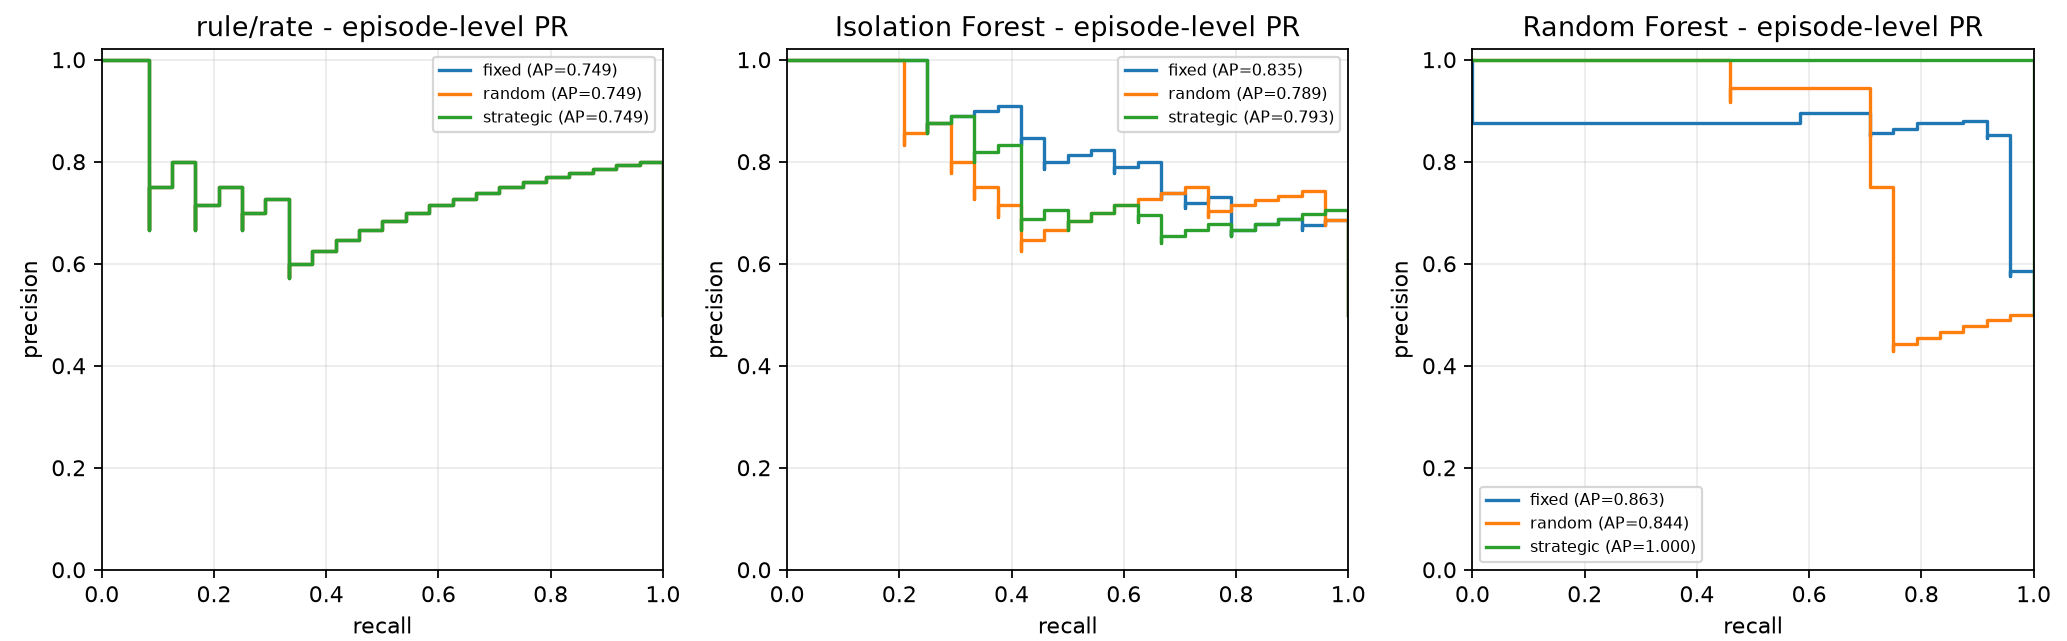
\includegraphics[width=\textwidth]{fig02_pr_curves.png}
\caption{Episode-level precision--recall curves on the frozen Zeek test set. Threshold-independent ranking and budget-constrained warning performance answer different questions.}
\label{fig:pr}
\end{figure}

\subsection{Temporal GRU and held-out-family performance}

The compact GRU produced no pre-onset alarms in any primary-seed policy. The uniform-random training corpus gave the strongest balance: F1 $=0.889$, PR-AUC $=0.965$, strict coverage $=0.833$, coverage-adjusted lead $=0.440$ s, and false-positive episode rate $=0.042$ (Table~\ref{tab:gru}). The strategic-policy GRU was most conservative, with zero false-positive episodes and strict coverage of 0.500.

\begin{table}[H]
\centering
\caption{Compact CPU GRU results on the validated Zeek sensor.}
\label{tab:gru}
\small
\begin{tabular}{@{}lrrrrrrrr@{}}
\toprule
Policy & Thr. & F1 & PR-AUC & Coverage & Strict & Lead (s) & FP rate & Pre-onset \\
\midrule
Fixed & .60 & .778 & .933 & .875 & .875 & .353 & .375 & 0 \\
Random & .75 & \metric{.889} & \metric{.965} & .833 & \metric{.833} & \metric{.440} & .042 & 0 \\
Strategic & .75 & .667 & .869 & .500 & .500 & .199 & \metric{.000} & 0 \\
\bottomrule
\end{tabular}
\end{table}

The held-out \texttt{slow\_ramp} family tested behavioural novelty rather than a claim of zero-day detection. The fixed-policy rate rule fell from 0.667 coverage on seen families to 0.000 on \texttt{slow\_ramp}; Isolation Forest coverage was 0.000 on both strata. Random Forest retained unseen-family coverage of 0.917 (fixed), 0.667 (random), and 1.000 (strategic). Thus, the learned supervised model transferred to the held-out behaviour more effectively than the rate-only rule.


\section{Ablation Studies and Replication}

\subsection{Ablation findings}

All feasible ablations required by the implemented methodology were executed on the same frozen test set:

\begin{itemize}
\item \textbf{Scenario policy:} no policy dominated simultaneously on strict coverage and false alarms. Fixed was most sensitive, strategic most conservative, and random was best balanced under the primary GRU.
\item \textbf{Temporal features:} removing five temporal features reduced rule coverage from 0.333 to 0.000 for every policy. Random Forest degraded more gracefully; fixed-policy PR-AUC changed from 0.863 to 0.681 and coverage from 0.958 to 0.875.
\item \textbf{Warning persistence:} requiring two consecutive alerting windows reduced Random Forest false-positive rates from 0.625/1.000/0.083 to 0.125/0.000/0.000 for fixed/random/strategic, but also reduced coverage from 0.958/0.833/1.000 to 0.667/0.500/0.625.
\item \textbf{Unseen scenario:} the rate rule collapsed on \texttt{slow\_ramp}; Random Forest retained 0.667--1.000 coverage.
\item \textbf{Observation source:} gateway and Zeek results differed materially, supporting source-separated reporting.
\end{itemize}

Graph-relation and topology-generalisation ablations were marked unavailable because no graph model and only one physical/logical topology were implemented. Reporting them as completed would not have been defensible.

\subsection{Independent second-seed replication}

The second collection used seed 20261116 under the identical protocol. It again contained 192 episodes, 3,840 gateway events, 7,688 Zeek connections, 100\% eligible bidirectional visibility, zero ambiguous joins, and complete episode coverage. This exact agreement supports the reproducibility of the capture and sensor pipeline.

\begin{table}[H]
\centering
\caption{Random Forest replication: strict coverage, false-positive episode rate, and pre-onset alarms.}
\small
\begin{tabular}{@{}lrrrrrr@{}}
\toprule
& \multicolumn{2}{c}{Strict coverage} & \multicolumn{2}{c}{FP rate} & \multicolumn{2}{c}{Pre-onset} \\
\cmidrule(lr){2-3}\cmidrule(lr){4-5}\cmidrule(lr){6-7}
Policy & Seed 1 & Seed 2 & Seed 1 & Seed 2 & Seed 1 & Seed 2 \\
\midrule
Fixed & .917 & .917 & .625 & .167 & 1 & 0 \\
Random & .833 & .542 & 1.000 & .042 & 0 & 0 \\
Strategic & .042 & .875 & .083 & .208 & 23 & 0 \\
\bottomrule
\end{tabular}
\end{table}

The strategic Random Forest's 23 pre-onset alarms in seed 1 did not recur in seed 2, so they cannot be treated as a stable property of the policy. Under the GRU, all six policy--seed configurations had zero pre-onset alarms. Strategic-policy GRU false-positive rates were the lowest in both seeds (0.000 and 0.042), while coverage increased from 0.500 to 0.750. Fixed-policy GRU coverage was 0.875 and 1.000; random-policy GRU coverage was 0.833 and 0.917. Consequently, the stable result is a sensitivity--conservatism trade-off, not a policy ranking.

\begin{figure}[H]
\centering
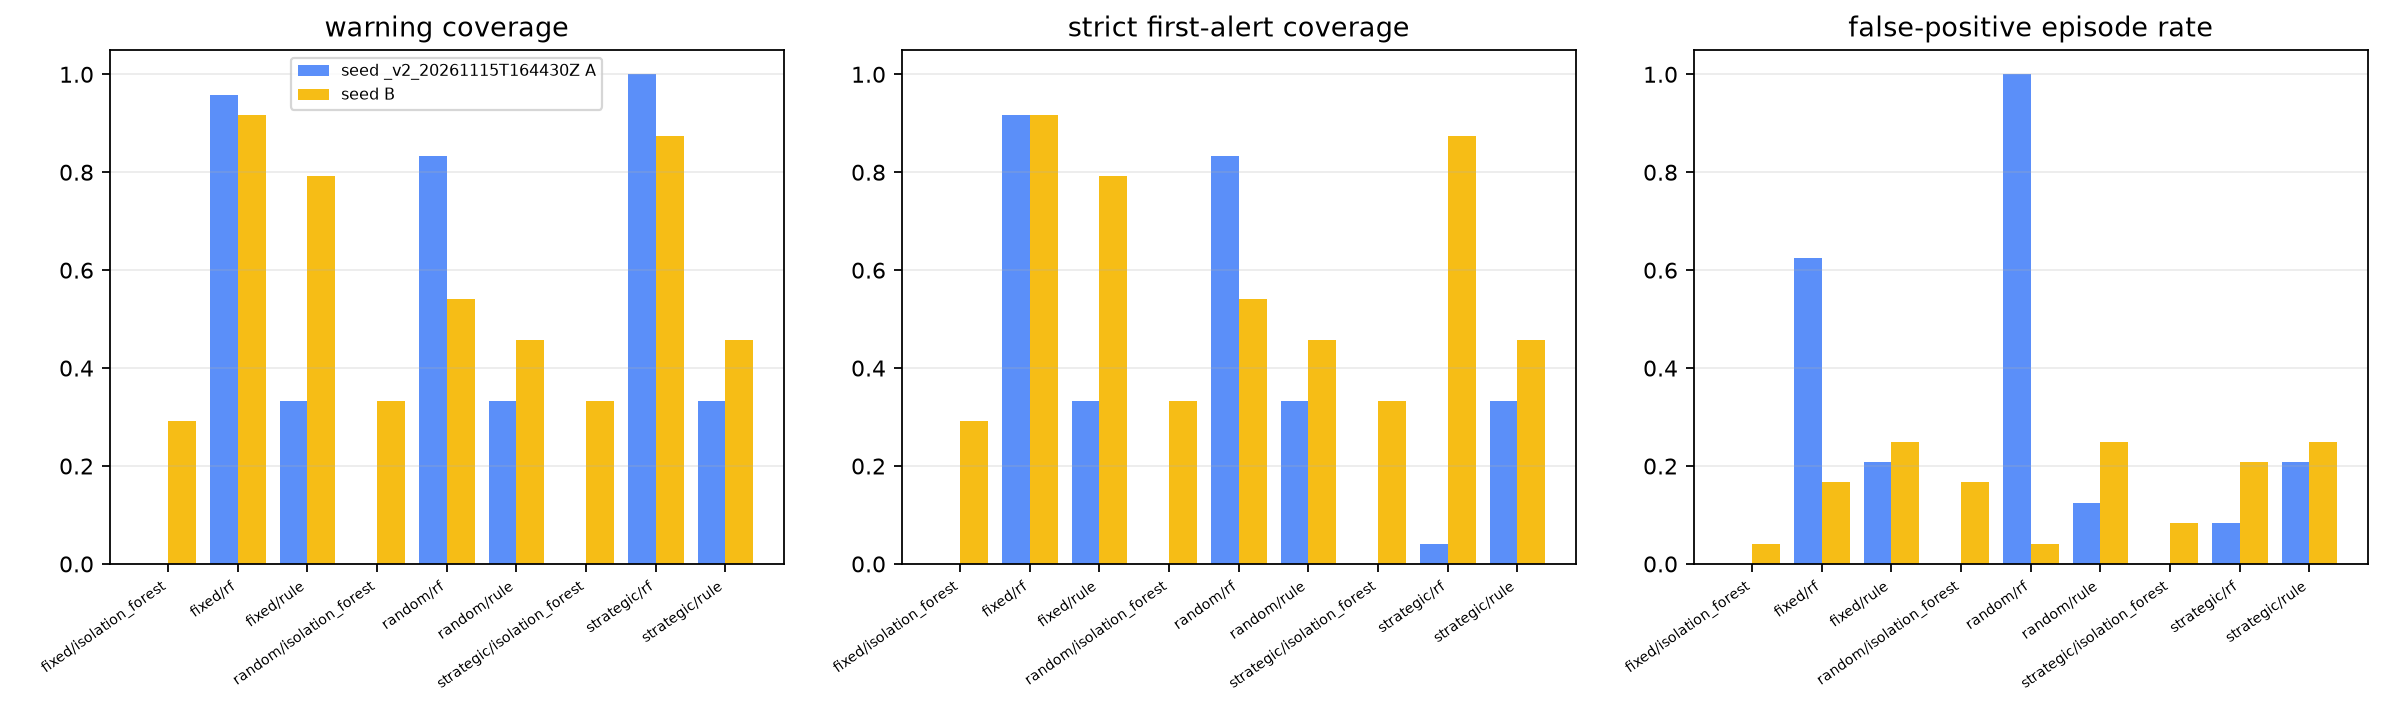
\includegraphics[width=\textwidth]{fig09_seed_comparison.png}
\caption{Configuration-level comparison of warning coverage, strict first-alert coverage, and false-positive episode rate across the two independent collections.}
\label{fig:seeds}
\end{figure}

\section{Critical Discussion}

The work successfully demonstrates a complete and auditable path from controlled network behaviour to pre-milestone warning. Its principal strength is methodological: controller ground truth, packet evidence, strict sensor validation, episode-level splitting, validation-only thresholds, source-separated reporting, and machine-verified numerical claims prevent several common forms of leakage and overstatement. The learned models also outperform the transparent rule on the held-out behaviour family, and the GRU provides useful warning performance without pre-onset firing.

The results also reveal limitations that affect interpretation. The profiles are synthetic and harmless; only two seeds and one topology were evaluated; 24 incident and 24 benign test episodes provide limited statistical power; the veth checksum artefact required a documented derived capture; and the strategic reward is a controller heuristic rather than detector feedback. The high Random Forest PR-AUC values reflect a deliberately bounded laboratory and must not be presented as real-world NIDS accuracy. The proposal's graph component and future-stage prediction were not implemented, so no graph or prediction claim is made. These limitations narrow the claim but do not weaken the reproducibility of the implemented experiment.

Relative to recent graph, transformer, and multi-stage intrusion-detection research, this study addresses a different task and evidence source. Published benchmark scores based on offline dataset rows are not numerically comparable with controller-timed warnings from a newly captured TCP trace. The contribution is therefore the controlled comparison of collection policies and the strict early-warning evaluation protocol.

\section{Reproducibility and Conclusion}

The main and replication run identifiers, full environment inventory, thresholds, per-window and per-episode metrics, figures with source-data JSON, ablation tables, checksums, sensor audits, and claim-to-artifact mappings are included with this report. The final verification recorded 53 passing tests, successful bytecode and shell-syntax checks, and 102 machine-checked report values with zero mismatches. Raw PCAPs are intentionally not stored in Git; the included reproduction instructions regenerate them in the isolated laboratory and apply the same fail-closed gate.

Phase 3 is complete as a reproducible implementation and exploratory experimental evaluation. The primary seed identifies the random-policy GRU as the strongest balanced operating point, while the replication shows that absolute policy rankings are not yet stable. Across both seeds, the strategic-policy GRU is consistently conservative, fixed-policy models tend to be more sensitive, and strict timing exposes conclusions that ordinary coverage alone would obscure. 

\begin{thebibliography}{9}
\small
\bibitem{graphinr}
P. Deepanramkumar and H. Sharmila A., ``GraphINR-IDS: Graph-Topology-Aware implicit neural reconstruction for zero-day intrusion detection in encrypted network traffic,'' \emph{Journal of King Saud University Computer and Information Sciences}, 2026, doi: \href{https://doi.org/10.1007/s44443-026-01260-x}{10.1007/s44443-026-01260-x}.

\bibitem{temporalflow}
T. J. Bala, A. Nag, C. Prabha, S. Biswas, A. K. Bairagi, M. Al-Maitah, and W. El-Shafai, ``Temporal flow-based dynamic graph neural network with robustness interpretation for DoS/DDoS IoT intrusion detection,'' \emph{Defence Technology}, 2026, doi: \href{https://doi.org/10.1016/j.dt.2026.06.002}{10.1016/j.dt.2026.06.002}.

\bibitem{multistage}
W. Afrifah, G. Epiphaniou, H. S. Lallie, and C. Maple, ``Multi-stage attack detection in IIoT supply chains using graph neural networks,'' \emph{International Journal of Information Security}, vol. 25, art. 176, 2026, doi: \href{https://doi.org/10.1007/s10207-026-01340-z}{10.1007/s10207-026-01340-z}.

\bibitem{alertprediction}
Z. Makki Nayeri and M. Rezvani, ``Alert prediction in computer networks using transformer-based temporal graph neural networks: Identifying the next victim,'' \emph{Journal of Network and Computer Applications}, vol. 249, art. 104455, 2026, doi: \href{https://doi.org/10.1016/j.jnca.2026.104455}{10.1016/j.jnca.2026.104455}.

\bibitem{dtgnn}
J. Yao and B. Koirala, ``Defense-Aware Temporal Graph Neural Network for fault-tolerant intrusion detection in IIoT--5G environments,'' \emph{Cluster Computing}, vol. 29, art. 319, 2026, doi: \href{https://doi.org/10.1007/s10586-026-06037-5}{10.1007/s10586-026-06037-5}.
\end{thebibliography}

\end{document}
